\chapter{实验} % (fold)
\label{cha:实验}
一般来说, 尽管隐私主成分分析有精确性保证, 但由于改进的三角机制减少了查询基与格点的个数, 因而\eqref{eq:误差项定义}中逼近误差$\eta_a$ 与离散化误差 $\eta_d$ 在理论上没有非平凡的上界, 这说明改进的三角机制难以达到原三角机制的精确性保证, 因而, 有必要通过实验来揭示改进的三角机制的精确性.

我们将改进的三角机制应用在以下公开发布的含有敏感信息的数据集中: 1) CRM\parencite{dataset:CRM}: 包括社会, 经济, 执法与犯罪的二十世纪九十年代美国社区数据. 2) CSN\parencite{dataset:CSN}: 提取自美国1994年人口普查的基本人口信息. 3) CTG\parencite{dataset:CTG}: 胎心监护图(包含胎心率和宫缩压力)的属性以及产科专家对监护图的分类. 4) PAM\parencite{dataset:PAM}: 用于运动感知的不同运动的传感器(包括地理位置, 加速度等)与心率数据. 5) PKS\parencite{dataset:PKS}: 从远程监护的早期Parkinson综合症患者的嗓音记录中提取的若干信息. 6)  WDBC\parencite{dataset:WDBC}: 从乳腺肿块细针穿刺的细胞学图像中提取的若干信息. 这些数据集涵盖了人口普查, 地理位置以及医疗领域, 是典型的需要进行隐私保护的数据集.
\renewcommand{\arraystretch}{1.5}
\begin{table}[hbtp]\centering
  \caption{实验使用数据集规模}\label{tab:数据集规模}
  \begin{tabular}{c|cc}
    \hline
    数据集 & 观测数($n$) & 属性个数 ($d$) \\
    \hline
    CRM & 1993 & 101 \\
    CSN & 100000 & 8 \\
    CTG & 2126 & 28 \\
    PAM & 19870 & 28 \\
    PKS & 5875 & 19 \\
    WDBC & 569 & 30 \\
    \hline
  \end{tabular}
\end{table}
\renewcommand{\arraystretch}{1}

表\ref{tab:数据集规模}给出了经过连续属性筛选, 缺失值清除, 退化列清除后的数据集规模信息. 由于本文假定数据库的域$\mathcal{X} = [-1, 1]^d$, 因此所有数据集的属性都进行了必要的正规化处理. 

\section{最坏情形误差} % (fold)
\label{sec:最坏情形误差}
为考察合成数据库回答光滑查询的最坏情形误差, 我们进行以下两组实验作为对比, 第一组实验采用保证$\epsilon$-差分隐私的改进三角机制(算法\ref{alg:改进的三角机制I}), 第二组实验采用保证$(\epsilon, \delta)$-差分隐私的三角机制(算法\ref{alg:改进的三角机制II}). 在两组实验中, 我们选取$\epsilon = 1, \delta = 10^{-3}$. 实验先输出合成数据库, 随后随机生成$10^4$个\eqref{eq:Gauss核函数线性组合}定义的 Gaussian 核函数线性组合
\[
  f(\mathbf{x}) = \sum_{j = 1}^J \alpha_j \exp\left(-\frac{\|\mathbf{x} - \mathbf{x}_j\|^2}{2\sigma^2}\right), 
\]
这里我们选择$J = 10$, 并对$j = 1, 2, \dots, J$, 随机生成$\mathbf{x_j} \sim U[-1, 1]$, $\boldsymbol{\alpha} \in U(A)$, 其中
\[
  A = \left\{(a_1, \dots, a_J)\colon a_j\ge 0, \sum_{j=1}^J \alpha_j = 1 \right\}.
\]
选择$\alpha_j > 0$是为了保证$f(\mathbf{x})$总是正的. 对于每一个生成的$f$, 我们将线性查询$q_f$分别作用在原始数据集$D$与合成数据集$D'$上, 并记算绝对误差与相对误差, $f(\mathbf{x})$总是正的也保证了相对误差是有意义的.  对这$10^4$组误差, 我们计算最坏情形的绝对误差与相对误差, 注意到当真实数据上的查询$q_f(D)$非常接近于$0$时, 对于可接受的绝对误差, 相对误差会非常大; 而对于$q_f(D)$比较大的情形, 相对误差更能反映算法的性能, 因此我们需要综合考察最坏相对误差与最坏绝对误差. 

实验分别选取\eqref{eq:Gauss核函数线性组合}中的$\sigma = 2, 4, 6, 8, 10$, 注意命题\ref{prop:Gauss 核函数线性组合的光滑性}揭示了$\sigma$与$K$的关系: $K = \sigma^2$. 我们在隐私主成分分析得到的椭球中抽取$C = 10^4$个格点, 每次实验重复$30$次, 并报告$10^4$个最坏情形误差的$30$次实验平均值与输出合成数据库所花费时间的最坏情形. 实验的计算环境为托管的刀片服务器, 其中CPU为两颗Intel®  Xeon®  X5650 处理器($6$核, $2.66$ GHz, $12$ M缓存), 内存使用$32$ GB 工作时钟为 $1333$ MHz 的DDR3 内存. 我们在算法\ref{alg:三角机制I}的瓶颈步骤 ------ 第\ref{alg:line:线性规划}步的线性规划求解中使用高效的IBM® ILOG CPLEX Optimization Studio\footnote{该软件为商业软件, 作者通过IBM® Academic Initiative 渠道获得该软件, 在其使用许可范围下在本文中以研究为目的进行进行并公开直接或衍生的计算结果. 使用许可参见\url{https://www-304.ibm.com/ibm/university/academic/pub/page/mem_software_guidelines}, 地址有效性于2014-05-10通过验证.}作为实现, 充分利用了CPU的计算资源. 在初期实验中, 我们发现, 与MATLAB自带的{\ttfamily linprog}相比, CPLEX为我们的线性规划问题带来了10 - 100倍的性能提升.

由表\ref{tab:保证epsilon-差分隐私的最坏情形误差与最坏运行时间}, 在保证$\epsilon$-差分隐私的情形下, 对于实验选定的数据集, 算法在十秒内输出合成数据库, 完全可以满足实际的速度需求. 对于不同数据集进行纵向对比可以发现, CSN误差表现是最好的, 回顾算法\ref{alg:改进的三角机制I}, 所有添加噪音的规模都关于$d$单调增, 关于$n$单调减, 噪音越大精确性越差; 而由表\ref{tab:数据集规模}知, CSN拥有最小的$\frac{d}{n}$比值, 因此这与理论的预期是一致的. 沿着$\sigma$方向进行横向对比, 除掉CRM与CTG数据集, 其余数据集的相对误差与绝对误差大体都呈现随着$\sigma$增大而下降的趋势, 注意到$K = \sigma^2$, 回顾表\ref{tab:算法性能指标与光滑阶数关系}, 查询的光滑度越大, 则三角机制越精确, 大部分数据集的实验结果与这一预期也是一致的. 最后, 我们强调对于$\epsilon$-差分隐私而言, 实验的一些数据集会由于规模不足而出现噪音过大的情形. 回顾算法\ref{alg:改进的三角机制I}与算法\ref{alg:保证epsilon差分隐私的子空间迭代算法}, 子空间迭代算法添加的噪音规模$\sigma$是整个改进三角机制中最大的: $\sigma = \frac{10\rho \sqrt{d}kL}{\epsilon}$, 事实上, 除了CSN外, 其余数据集的$\sigma$均大于$1$甚至接近$10$的量级, 注意到$D\in\left([-1,1]^d\right)^n$, 因而方差阵$\mathbf{A}(D)\in[-1, 1]^{d\times d}$, 故$\sigma$如果大于$1$则隐私主成分分析难以保证其精度. 这也解释了除了CSN数据集外其余数据集性能较差的现象. 

\renewcommand{\arraystretch}{1.5}
\begin{table}[hbtp]\centering
	\caption{改进的三角机制I在各数据集上的最大误差与最坏运行时间}
	\label{tab:保证epsilon-差分隐私的最坏情形误差与最坏运行时间}
	\begin{tabular}{c|c|ccccc|c}
		\hline
		 \multirow{2}*{数据集} & \multirow{2}*{误差类型} & \multicolumn{5}{c|}{$\sigma$} & \multirow{2}*{时间(秒)}\\\cline{3-7}
		   & & 2 & 4 & 6 & 8 & 10 & \\
		\hline
		\multirow{2}*{CRM} & 绝对 & 0.002&0.010&0.070&0.074&0.041& \multirow{2}{*}{2.5} \\
		 & 相对 & 1.796&0.085&0.166&0.122&0.056& \\
		\hline
		\multirow{2}*{CSN} & 绝对 & 0.053&0.011&0.011&0.009&0.003& \multirow{2}{*}{1.7} \\
		 & 相对 & 0.174&0.015&0.013&0.010&0.003& \\
		\hline
		\multirow{2}*{CTG} & 绝对 & 0.053&0.199&0.031&0.054&0.056& \multirow{2}{*}{0.7} \\
		 & 相对 & 0.488&0.360&0.041&0.062&0.061& \\
		\hline
		\multirow{2}*{PAM} & 绝对 & 0.239&0.278&0.175&0.107&0.065& \multirow{2}{*}{0.9} \\
		 & 相对 & 0.848&0.390&0.205&0.117&0.069& \\
		\hline
		\multirow{2}*{PKS} & 绝对 & 0.075&0.030&0.049&0.023&0.015& \multirow{2}{*}{0.7} \\
		 & 相对 & 0.326&0.044&0.058&0.026&0.016& \\
		\hline
		\multirow{2}*{WDBC} & 绝对 & 0.049&0.167&0.154&0.041&0.024& \multirow{2}{*}{0.7} \\
		 & 相对 & 0.355&0.280&0.194&0.047&0.026& \\	
		 \hline
	\end{tabular}
\end{table}
\renewcommand{\arraystretch}{1}

表\ref{tab:保证epsilon,delta-差分隐私的最坏情形误差与最坏运行时间}的误差在横向对比与纵向对比上的结果与表\ref{tab:保证epsilon-差分隐私的最坏情形误差与最坏运行时间}是一致的, 此处不表.  比较表\ref{tab:保证epsilon,delta-差分隐私的最坏情形误差与最坏运行时间}与表\ref{tab:保证epsilon-差分隐私的最坏情形误差与最坏运行时间}可以发现, 改进的三角机制II与改进的三角机制I相比, 在所有数据集上误差均有明显的改善. 与算法\ref{alg:改进的三角机制I}对比, 算法\ref{alg:改进的三角机制II}的最大噪音规模也是隐私主成分分析的噪音, 回顾算法\ref{alg:保证epsilon,delta差分隐私的子空间迭代算法}, 此时$\sigma = \frac{\rho\sqrt{4kL\log(1/\delta)}}{\epsilon}$, 对于大部分数据集而言, 这样的$\sigma$与算法\ref{alg:保证epsilon差分隐私的子空间迭代算法}的$\sigma$相比是可以接受的, 即噪音规模约为$o(1)$, 此时由于隐私主成分分析更为精确, 算法的误差也较表\ref{tab:保证epsilon-差分隐私的最坏情形误差与最坏运行时间}有明显改善. 此外, 在$(\epsilon, \delta)$-差分隐私下, 算法可以接受更大的基函数个数$R$, 因而三角机制II运行时间较三角机制I长, 实验结果与这一预期也是一致的. 
\renewcommand{\arraystretch}{1.5}
\begin{table}[hbtp]\centering
	\caption{改进的三角机制II在各数据集上的最大误差与最坏运行时间}
	\label{tab:保证epsilon,delta-差分隐私的最坏情形误差与最坏运行时间}
	\begin{tabular}{c|c|ccccc|c}
		\hline
		 \multirow{2}*{数据集} & \multirow{2}*{误差类型} & \multicolumn{5}{c|}{$\sigma$} & \multirow{2}*{时间(秒)}\\\cline{3-7}
		   & & 2 & 4 & 6 & 8 & 10 & \\
		\hline
		\multirow{2}*{CRM} & 绝对 & 0.000&0.070&0.059&0.111&0.097& \multirow{2}{*}{6.5} \\
		 & 相对 & 0.616&0.481&0.141&0.184&0.134& \\
		\hline
		\multirow{2}*{CSN} & 绝对 & 0.039&0.026&0.008&0.008&0.003& \multirow{2}{*}{7.2} \\
		 & 相对 & 0.095&0.035&0.009&0.008&0.003& \\
		\hline
		\multirow{2}*{CTG} & 绝对 & 0.036&0.130&0.062&0.064&0.033& \multirow{2}{*}{10.5} \\
		 & 相对 & 0.342&0.234&0.082&0.075&0.036& \\
		\hline
		\multirow{2}*{PAM} & 绝对 & 0.190&0.205&0.164&0.089&0.071& \multirow{2}{*}{12.8} \\
		 & 相对 & 0.693&0.296&0.194&0.098&0.075& \\
		\hline
		\multirow{2}*{PKS} & 绝对 & 0.115&0.033&0.060&0.025&0.023& \multirow{2}{*}{5.4} \\
		 & 相对 & 0.440&0.049&0.071&0.028&0.024& \\
		\hline
		\multirow{2}*{WDBC} & 绝对 & 0.063&0.213&0.089&0.069&0.042& \multirow{2}{*}{10.7} \\
		 & 相对 & 0.452&0.360&0.113&0.079&0.046& \\	
		 \hline
	\end{tabular}
\end{table}
\renewcommand{\arraystretch}{1}
% section 最坏情形误差 (end)
\section{误差与部分参数关系} % (fold)
\label{sec:误差与部分参数关系}
改进的三角机制有许多外生参数, 本节选取了两个数据集, 探讨最坏情形绝对误差与椭圆半径缩放系数$\kappa$, 主成分分析输出维数$k$的关系. 

\paragraph{椭圆半径缩放系数$\kappa$} % (fold)
\label{par:椭圆半径缩放系数_kappa_}
回顾算法\ref{alg:改进的三角机制I}, 特征值的平方根$\sqrt{\boldsymbol{\lambda}}$决定了椭球各半轴长的相对比例, 系数$\kappa$决定了用来抽取格点的椭球的轴长单位, 注意到高维空间的椭球体积大部分集中在球壳附近, 因此, 如果椭球太小或者太大, 都会使得椭球中的点与原始数据集接近的可能性降低, 图\ref{fig:CSN数据集最坏绝对误差与椭圆半径缩放系数_kappa}所示的实验结果对这一观点提供了支持. 注意到算法本身的随机性使我们难以呈现一个清晰的趋势.
% paragraph 椭圆半径缩放系数_kappa_ (end)
\begin{figure}[hbtp]\centering
  \caption{CSN数据集最坏绝对误差与椭圆半径缩放系数$\kappa$, 隐私设定为$\epsilon$-差分隐私, $\epsilon = 1, C = 10^4, R = 50, L = 10, k = 2$,  每次实验重复10次取平均值}\label{fig:CSN数据集最坏绝对误差与椭圆半径缩放系数_kappa}
  % \vskip\baselineskip % This is a dirty hack so just remove it if the figure is OK.
  \makeatletter
  \ifpkuthssextra@opt@colorlinks
  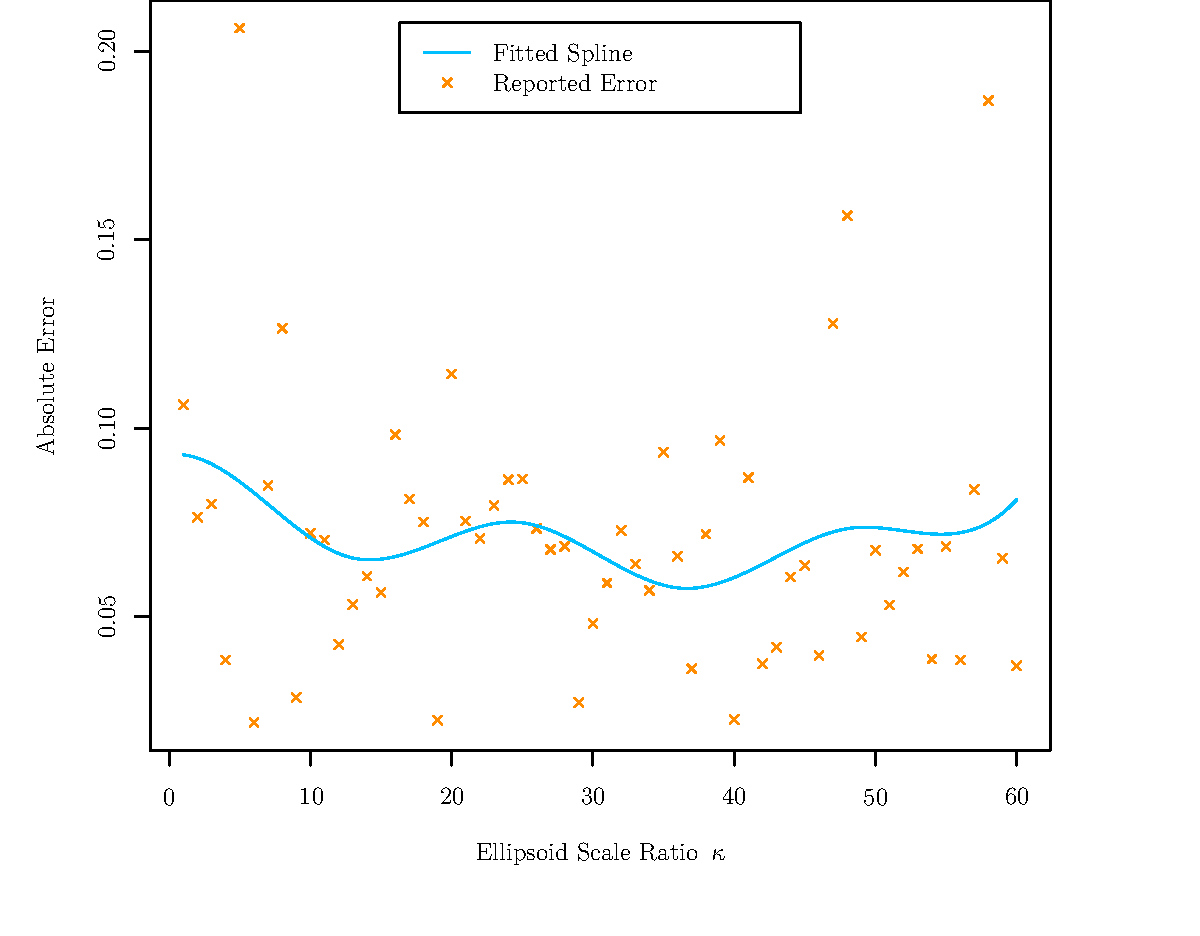
\includegraphics[width=140mm]{fig/fig_CSN.pdf}
  \else
  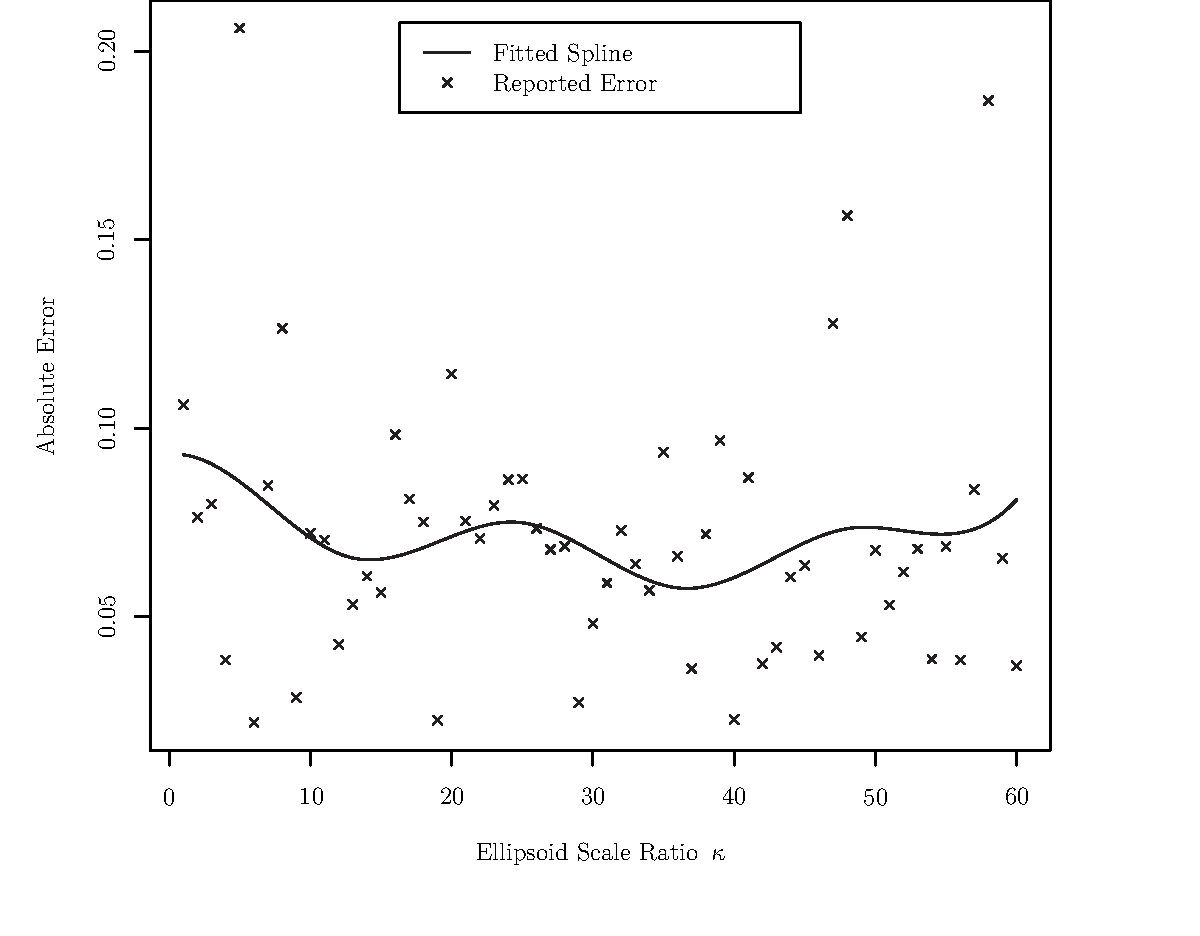
\includegraphics[width=140mm]{fig/fig_CSN_bw.pdf}
  \fi
  \makeatother
\end{figure}
\paragraph{隐私主成分分析输出维度$k$} % (fold)
\label{par:隐私主成分分析输出维度_k_}
输出维度$k$对算法精确性的影响是微妙的, 一方面, 增大$k$可以更好地概括原始数据集的分布信息, 但另一方面, 由算法\ref{alg:保证epsilon,delta差分隐私的子空间迭代算法}, $k$增大每一步增加的噪音也会相应增大, 从图\ref{fig:CRM数据集最坏绝对误差与隐私主成分分析输出维数_k}来看, $k$的增加对误差的影响方向并不确定. 
% paragraph 隐私主成分分析输出维度_k_ (end)
\begin{figure}[hbtp]\centering
  \caption{CRM数据集最坏绝对误差与隐私主成分分析输出维数$k$, 隐私设定为$(\epsilon, \delta)$-差分隐私, 其中$C=10^4, R = 102, L = 10, \kappa = 7$, 每次实验重复10次取平均值 }\label{fig:CRM数据集最坏绝对误差与隐私主成分分析输出维数_k}
  % \vskip\baselineskip % This is a dirty hack so just remove it if the figure is OK.
  \makeatletter
  \ifpkuthssextra@opt@colorlinks
  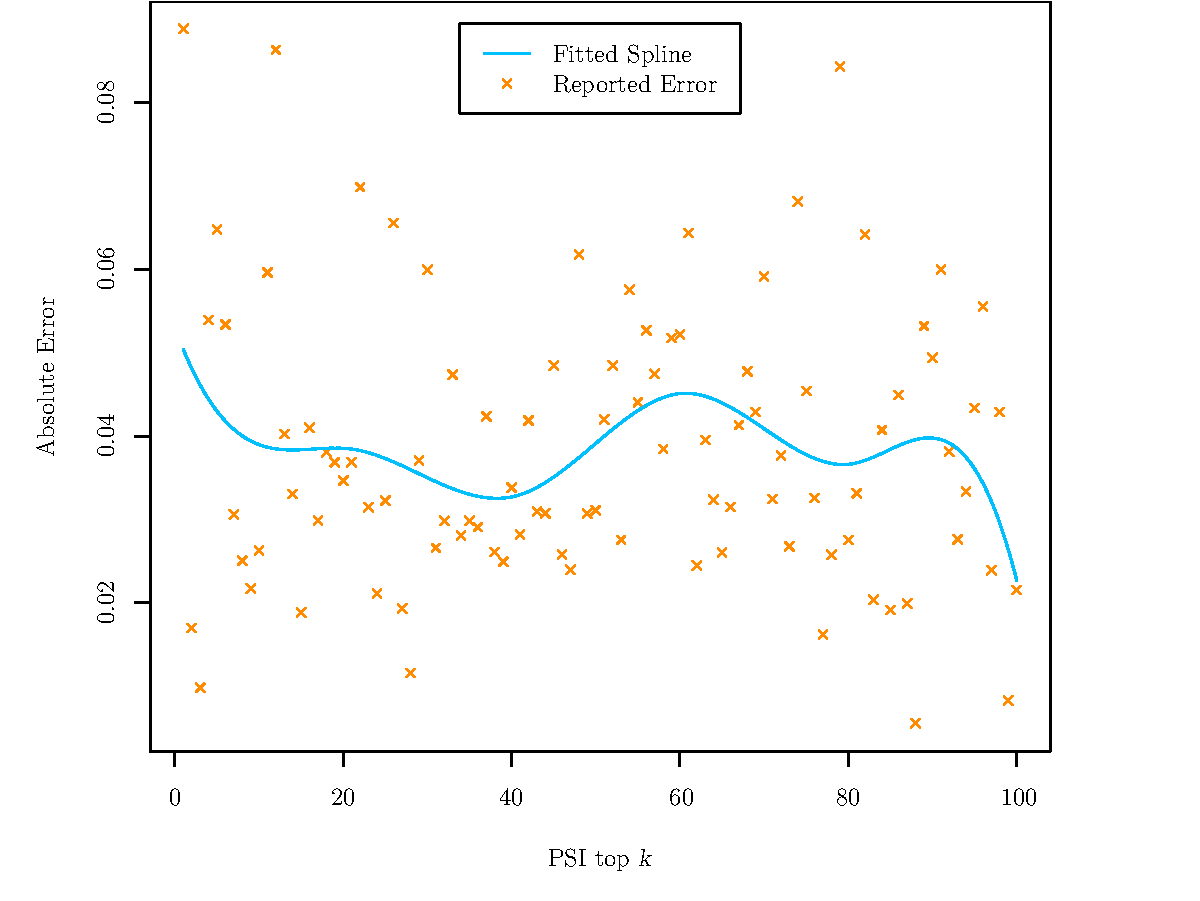
\includegraphics[width=140mm]{fig/fig_CRM.pdf}
  \else
  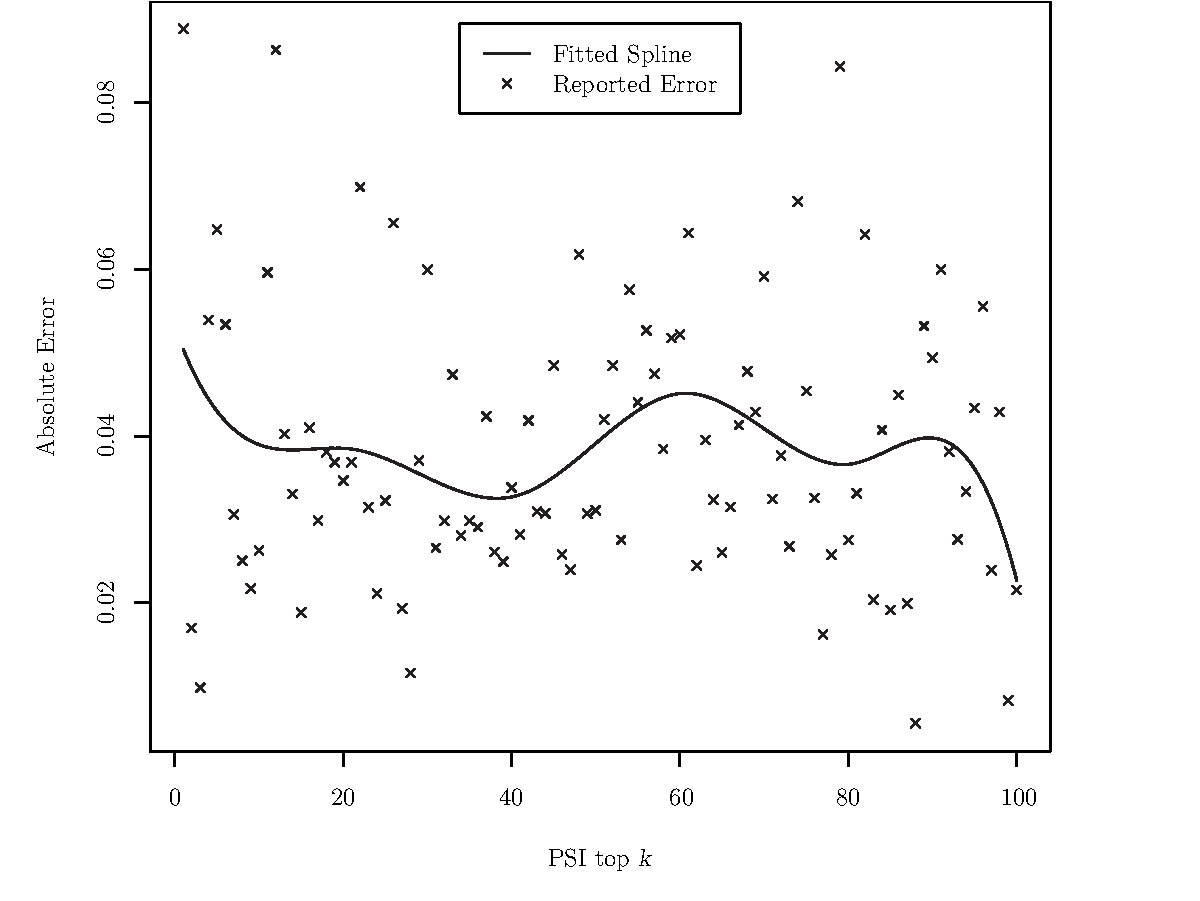
\includegraphics[width=140mm]{fig/fig_CRM_bw.pdf}
  \fi
  \makeatother
\end{figure}
% section 误差与部分参数关系 (end)
% chapter 实验 (end)